%%%%%%%%%%%%%%%%%%%%%%%%%%%%%%%%%%%%%%%%%%%%%%%%%%%%%%%%%%%%%%%%%%%%%%%%
%    INSTITUTE OF PHYSICS PUBLISHING                                   %
%                                                                      %
%   `Preparing an article for publication in an Institute of Physics   %
%    Publishing journal using LaTeX'                                   %
%                                                                      %
%    LaTeX source code `ioplau2e.tex' used to generate `author         %
%    guidelines', the documentation explaining and demonstrating use   %
%    of the Institute of Physics Publishing LaTeX preprint files       %
%    `iopart.cls, iopart12.clo and iopart10.clo'.                      %
%                                                                      %
%    `ioplau2e.tex' itself uses LaTeX with `iopart.cls'                %
%                                                                      %
%%%%%%%%%%%%%%%%%%%%%%%%%%%%%%%%%%
%
%
% First we have a character check
%
% ! exclamation mark    " double quote  
% # hash                ` opening quote (grave)
% & ampersand           ' closing quote (acute)
% $ dollar              % percent       
% ( open parenthesis    ) close paren.  
% - hyphen              = equals sign
% | vertical bar        ~ tilde         
% @ at sign             _ underscore
% { open curly brace    } close curly   
% [ open square         ] close square bracket
% + plus sign           ; semi-colon    
% * asterisk            : colon
% < open angle bracket  > close angle   
% , comma               . full stop
% ? question mark       / forward slash 
% \ backslash           ^ circumflex
%
% ABCDEFGHIJKLMNOPQRSTUVWXYZ 
% abcdefghijklmnopqrstuvwxyz 
% 1234567890
%
%%%%%%%%%%%%%%%%%%%%%%%%%%%%%%%%%%%%%%%%%%%%%%%%%%%%%%%%%%%%%%%%%%%
%

%AIP Reprint Class%%%%%%%%%%%%%%%%%%%%%%%%%%%%%%%%%%%%%%%%%%%%%%%%%%%%%%%%%%%%%%%%%%%%%%%%%%%%%
\documentclass[aps,prl,amsmath,amssymb,reprint,superscriptaddress]{revtex4-1} %preprint version
\usepackage{graphicx}% Include figure files
\usepackage{dcolumn}% Align table columns on decimal point
\usepackage{bm}% bold math
\usepackage{epstopdf}

    \renewcommand{\topfraction}{0.9}    % max fraction of floats at top
    \renewcommand{\bottomfraction}{0.8}    % max fraction of floats at bottom
    \setcounter{topnumber}{2}
    \setcounter{bottomnumber}{2}
    \setcounter{totalnumber}{4}     % 2 may work better
    \setcounter{dbltopnumber}{2}    % for 2-column pages
    \renewcommand{\dbltopfraction}{0.9}    % fit big float above 2-col. text
    \renewcommand{\textfraction}{0.07}    % allow minimal text w. figs
    \renewcommand{\floatpagefraction}{0.7}    % require fuller float pages
    \renewcommand{\dblfloatpagefraction}{0.7}    % require fuller float pages
    \setlength{\abovecaptionskip}{5pt}
    \setlength{\belowcaptionskip}{5pt}
    \setlength{\parskip}{0pt}
    \setlength{\textfloatsep}{5pt} 

%%%%%%%%%%%%%%%%%%%%%%%%%%%%%%%%%%%%%%%%%%%%%%%%%%%%%%%%%%%%%%%%%%%%%%%%%%%%%%%%%%%%%%%%%%%%%%%%%%

%IOP preprint class %%%%%%%%%%%%%%%%%%%%%%%%%%%%%%%%%%%%%%%%%%%%%%%%%%%%%%%%%%%%%%%%%%%%%%%%%%%%%%
%\documentclass[12pt]{iopart}
%\newcommand{\gguide}{{\it Preparing graphics for IOP journals}}
%Uncomment next line if AMS fonts required
%\usepackage{iopams}
%\usepackage{graphicx}
%\usepackage{epstopdf}  
%%%%%%%%%%%%%%%%%%%%%%%%%%%%%%%%%%%%%%%%%%%%%%%%%%%%%%%%%%%%%%%%%%%%%%%%%%%%%%%%%%%%%%%%%%%%%%%%%%
%Slava's inserts %%%%%%%%%%%%%%%%%%%%%%%%%%%%%%%%%%%%%%%%%%%%%%%%%%%%%%%%%%%%%%%%%%%%%%%%%%%%%%
%\usepackage{amsfonts}
%\usepackage{amssymb}

%\newcommand{\ptt}[1]{\frac{\partial#1}{\partial t}}
%\newcommand{\vvec}{\mathbf{v}}
%\newcommand{\Bvec}{\mathbf{B}}
%\newcommand{\Evec}{\mathbf{E}}
%\newcommand{\Jvec}{\mathbf{J}}
%\newcommand{\Avec}{\mathbf{A}}
%%%%%%%%%%%%%%%%%%%%%%%%%%%%%%%%%%%%%%%%%%%%%%%%%%%%%%%%%%%%%%%%%%%%%%%%%%%%%%%%%%%%%%%%%%%%%%%%%%

\begin{document}
\title{Observation of turbulent intermittency scaling with magnetic helicity in an MHD plasma wind-tunnel}

\author{D.A. Schaffner}
\author{A. Wan}
\author{M.R. Brown}
\affiliation{Swarthmore College, Swarthmore, PA, USA}
\date{\today}
\begin{abstract}
The intermittency in turbulent magnetic field fluctuations has been observed to scale with the amount of magnetic helicity injected into an experimental flux rope plasma. A selectively decayed Taylor state is created in the wind-tunnel configuration of the Swarthmore Spheromak Experiment using a magnetized plasma gun that can inject plasma of varying levels of helicity into the chamber. The level of intermittency is determined by finding the flatness of the probability distribution function of increments for magnetic pickup coil fluctuations, $\dot{B}(t)$. The intermittency is observed to increase with the injected helicity while the spectral index in the inertial range of the turbulence is unaffected by this variation. Evidence for the role of current sheets and reconnection sites in the generation of this intermittency is provided, but the true nature of the observed intermittency remains unknown.
\end{abstract}

\maketitle

Varying levels of intermittency~\cite{frisch95} in magnetic fluctuations have been observed in many different turbulent plasmas in both space and laboratory settings. Differences in magnetic intermittent character have been seen between fast and slow solar wind turbulence~\cite{sorrisovalvo99}, at varying spatial scales in the solar wind~\cite{wan12}, and between different confinement regimes in laboratory experiments, particular in reverse field pinches~\cite{sorrisovalvo01,marrelli05}. Simulation generated intermittency in MHD turbulence~\cite{Greco08,Greco09,Wan09,Servidio11b} compared with {\it in situ} measurements in the solar wind has suggested a link between such non-Gaussian fluctuations and the presence of current sheets or reconnection layers. Since magnetic helicity of a plasma is reflective of the twistedness or knottedness of the magnetic field, a scan of magnetic helicity can be used in order to vary the magnetic field structure and potentially modify the character of current sheets in the plasma. A novel experiment was developed on the MHD wind-tunnel configuration of the Swarthmore Spheromak Experiment (SSX)~\cite{Gray13,schaffner14} to explore this possible relationship between the observed intermittency in magnetic fluctuations and the magnetic helicity of the plasma. Given the nature of the plasma source on SSX, magnetic helicity injection can be very finely controlled and thus resulting changes in turbulent characteristics---including both spectra and intermittency---can be carefully examined.

%The study of magnetic turbulence in laboratory experiment and in space plasmas has been conducted using a multitude of approaches including the construction and analysis of power spectra, correlations and probability distribution functions for both temporal and spatial datasets~\cite{deWit13}. Much focus has been placed on studying power spectra, or really, the rate of transfer of energy from large scales to small scales reflected in the spectral index, as this quantity has the most intuitive physical reason and firmest connection to the Kolmogorov theory of fluid turbulence. However, examination of power spectra follows only one thread of insight into the characteristics that make up a turbulent plasma. The role of intermittency in turbulence theory has developed alongside spectral theory in fluid mechanics~\cite{frisch95} and has become an integral aspect of turbulence analysis in both space~\cite{Greco08,Greco09,Wan09} and laboratory plasmas~\cite{carter06,serianni07}. 

This paper presents the results of an experimental scan which establishes a connection between a controllable experimental quantity---magnetic helicity---and a turbulent characteristic---intermittency. As the amount of injected magnetic helicity is increased, the measured flatness or kurtosis of the distribution of fluctuations in a magnetic pickup coil, $\dot{B}(t)$, are also shown to increase ranging from near Gaussian (F$\sim 5$) to values of F $>$ 30. In contrast, the power-law behavior of the spectra of these fluctuations are shown to be unaffected by this variation in helicity as shown by the power-law fit spectral indices. The scan is conducted on the wind-tunnel configuration of the Swarthmore Spheromak Experiment which consists of an 86cm long by 15.5cm wide cylindrical copper flux conserver into which a plasma gun injects dense, highly magnetized ($\sim 1\times 10^{15} cm^{-3}, \sim 5kG$) spheromak-shaped plasma self-organizes by tilting and twisting into a Taylor state~\cite{Gray13,Matthaeus80,Taylor86}. There is no guide or vacuum field in the chamber so the magnetic field embedded in the plasma are completely dynamical. 

%The injected magnetic helicity of the plasma can be modified by setting the amount of flux through the plasma gun using a coaxial magnetic coil. Power spectra and probability density functions of increments are constructed using fluctuation magnetic data extract from pickup coils ($\dot{B}$ probes) inserted radially into the flux conserver at the midplane. While power-law fits to the power spectra show no scaling with the change in helicity, the turbulent intermittency, as indicated by the calculated flatness of the PDFs, increases with the helicity with flatness values ranging from 

%In a laboratory plasma, Gray, {\it et al.}~\cite{Gray13} recently reported on the observation of a long-lived helical flux rope called a Taylor double-helix in the SSX MHD wind tunnel.  The Taylor double-helix is the natural relaxed state of MHD plasma confined in a long, perfectly conducting cylinder~\cite{Taylor86}.  In the case of an infinite cylinder of radius $a$, the minimum energy state has a helical pitch of $ ka = 1.234$, where k is the wave number associated with the axis of the cylinder.

%In the SSX experiments, a magnetized plasma gun launches a magnetized plasma plume into a long flux conserving cylinder.  The plasma rapidly relaxes to the double-helix state in about 1 Alfv\'en crossing time and subsequently decays resistively.  Gray, {\it et al.}~\cite{Gray13} postulated that the physics of selective decay was at play as the initially turbulent plasma relaxed to the double-helix state.  The selective decay hypothesis posits that the energy selectively decays relative to the magnetic helicity because the energy spectra peaks at higher wave numbers, where dissipation is higher~\cite{Matthaeus80}.  The wind tunnel's minimum energy state possesses $ka = 1.292$, which is within 5\% of the infinite cylinder's $ka = 1.234$. 

%\begin{figure}[!htbp]
%\centerline{
%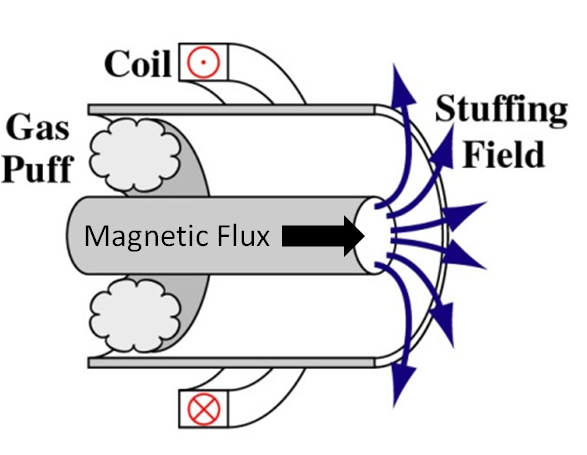
\includegraphics[width=8.5cm]{plasmagun_closeup2.png}}
%\caption{\label{fig:plasmagun_closeup2} Diagram of the plasma gun attached to one end of the copper flux conserver in SSX. The diagram shows how the magnetic flux in the core of the gun is modified by adjusting the current in the coil outside of the gun which sets up the stuffing field.}
%\end{figure}

The injection of magnetic helicity into the plasma is a natural consequence of the formation procedure for a plasma gun. Magnetic helicity,
%
\begin{equation}
K_{B} = \int A \cdot B dV
\label{eq:helicity_th}
\end{equation}
%
is a measure of the amount of twistedness of the magnetic field lines and can be expressed in terms of magnetic flux squared (i.e. units of $Wb^{2}$). This quantity can be recast in a more experimentally relevant quantity, 
%
\begin{equation}
K_{B} = \int \Phi V_{gun} dt
\label{eq:helicity_exp}
\end{equation}
%
where $\Phi$ is the magnetic flux penetrating the plasma gun core and $V_{gun}$ is the voltage drop across the gun gap. This is the form of the helicity that is calculated and reported in this paper. Since the plasma forms under the assumption of selective decay (conservation of magnetic helicity)~\cite{Gray13}, it is further assumed that the amount of helicity injected by the gun is conserved and present in the plasma under observation. Though the voltage across the gun gap is recorded for the entire duration of the shot, only the first $20 \mu s$ after initial trigger of the capacitor banks and breakdown of the hydrogen gas are used to estimate the injected helicity. Beyond $20 \mu s$, the voltage measurement is significantly affected by breaking field lines during spheromak formation. Though it is assumed that helicity injection is nearly constant for the duration of the discharge, the values of helicity reported here again those from integrating the first $20 \mu s$ after the initial trigger.

\begin{figure}[!htbp]
\centerline{
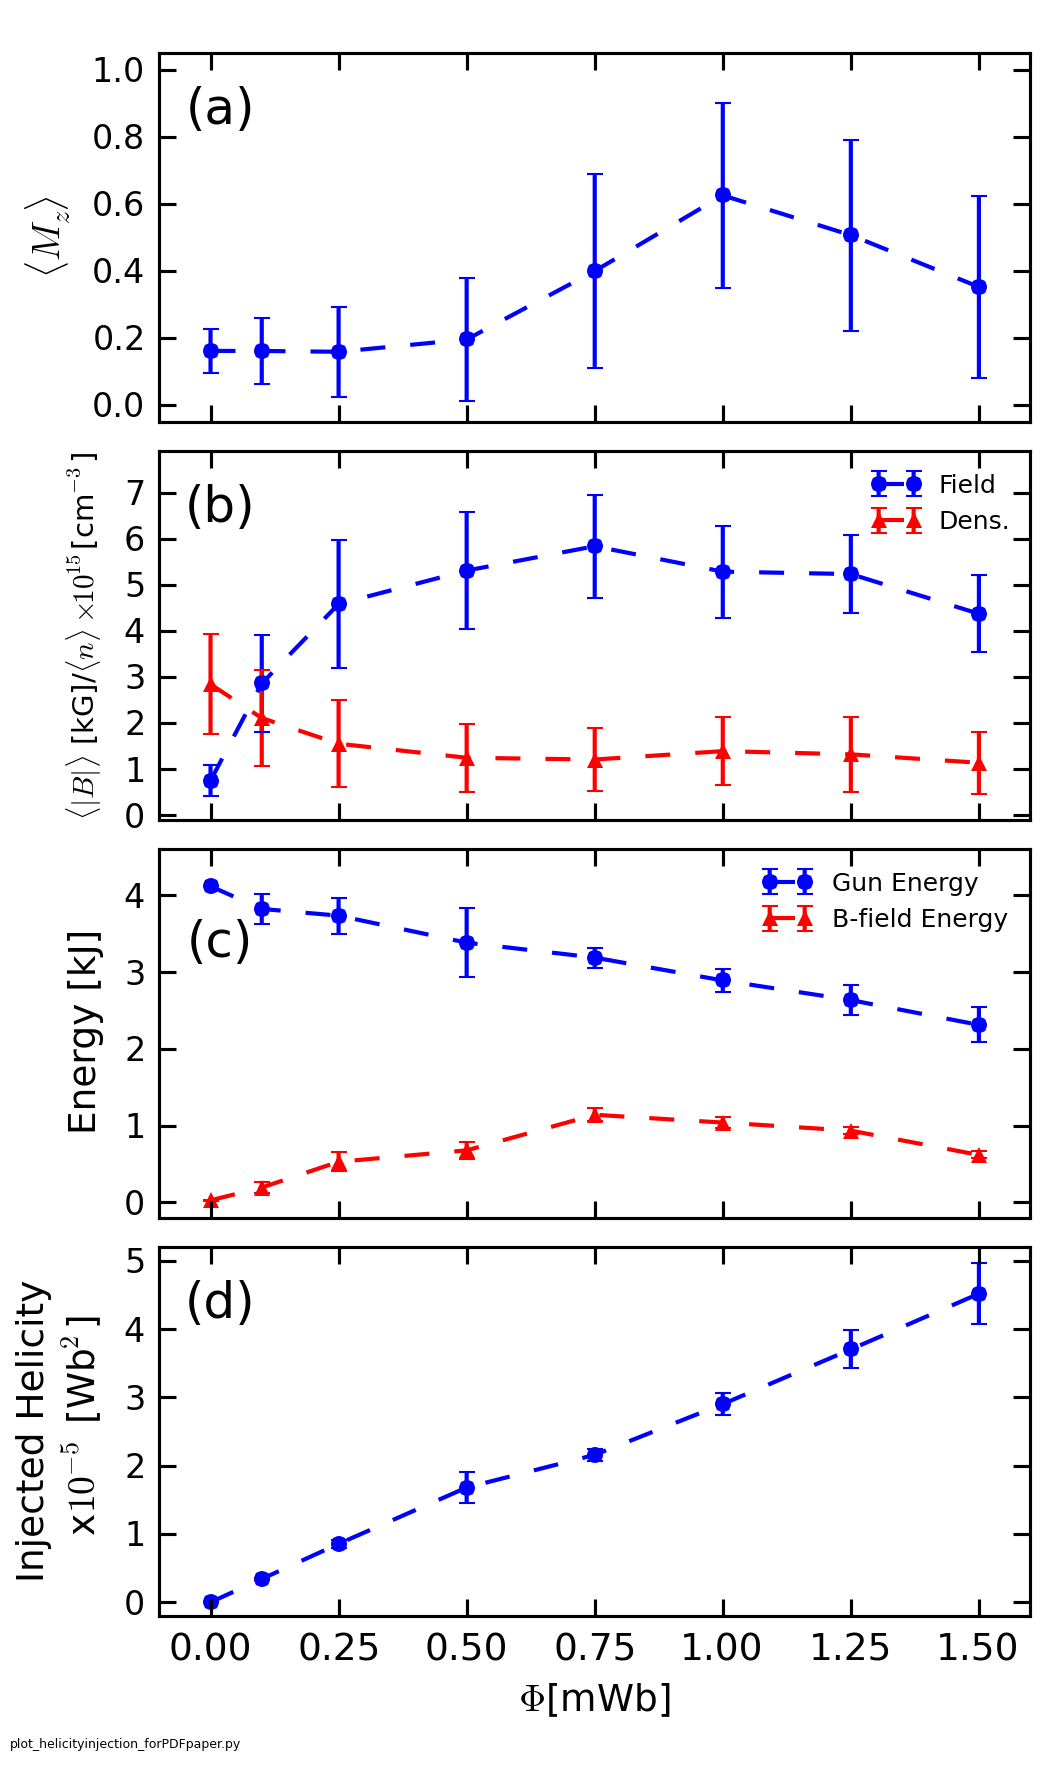
\includegraphics[width=8.5cm]{helicity_scaling.png}}
\caption{\label{fig:helicity_scaling} (a) Average magnetic field magnitude over the equilibrium epoch (40-60$\mu s$), (b) injected gun energy and volume integrated magnetic field energy, and (c) amount of helicity injected in the first $20 \mu s$ after discharge trigger as a function of magnetic flux in gun core. Error bars for all three plots indicate the standard deviation in values of field and potential (and propagated into energy and helicity) over the time spans discussed in the text and shot number.}
\end{figure}

The gun voltage is set by a combination of the gun circuit and breakdown physics, but typically does not vary given a particular capacitor charge setting and gas input delay time. Thus, by Eqn.~\ref{eq:helicity_exp}, the injected helicity is modified by the amount of magnetic flux penetrating the gun core. This flux, in turn, is set by the the amount of current run through the stuffing coil. The stuffing coil produces magnetic field parallel to the gun axis using a capacitor discharge circuit, but with a much longer timescale than the gun discharge. Because the stuffing coil discharge is much slower, rather than modify the discharge voltage to vary the magnetic field in the gun, the field is set by changing the timing of when the gun fires relative to the stuffing coil. Thus, changes in flux, and consequently helicity are adjusted by changing the timing delay of the gun trigger.

The flux can be ranged from 0.0 to 1.5mWb which, given a gun voltage of approximately 900V, yields an injected helicity range of 0 to 5$ \times 10^{-5} Wb^{2}$. As indicated in Figure~\ref{fig:helicity_scaling}(c), the injected helicity scales linearly with the varied magnetic flux. Figure~\ref{fig:helicity_scaling}(a) and (b) show how the average magnetic field in the center of the chamber and the energy changes with magnetic flux. The magnetic field is determined from time-integration of a three-axis magnetic pickup probe timeseries about 1cm off of the central cylindrical axis, and is time averaged from 40 to 60$\mu s$. As Figure~\ref{fig:helicity_scaling}(a) shows, this value increases initially with flux, but saturates at a value around $5kG$ for most flux settings. The gun energy is found by integrating the power, $P = I_{gun}V_{gun}$, from 0.0 to 60.0$\mu s$ and represents the maximum amount of energy that can be delivered into the plasma. This value begins around $4kJ$ which is about half of the possible circuit energy based on the 1mF, 4.0kV capacitor circuit, and decreases steadily with increasing flux as shown with blue in Fig.~\ref{fig:helicity_scaling}(b). The amount of energy that actually gets deposited into the magnetic fields is indicated by red in Fig.~\ref{fig:helicity_scaling}(b), and as would be expected, follows a similar trend as the field magnitude. This energy is calculated by finding the energy density, $B^{2}/2\mu_{0}$, for at 16 radial points in the chamber and integrating over the volume at each location. Comparison of the three sub-figures in Figure~\ref{fig:helicity_scaling} demonstrate the ability to modify the helicity of the plasma without significantly changing the total energy content.

Two turbulence analysis techniques, power spectra and the probability distribution (PDF) of increments are constructed using the magnetic pickup coil timeseries or $\dot{B}$ data. Since the probe is fabricated using a single 3mm wide loop, the $\dot{B}(t)$ signal has the best temporal resolution and bit-depth (65MHz sampling and 14-bit dynamic range) and is used directly in the analysis rather than converting the timeseries to $B(t)$ by integration. In frequency space, the $\dot{B}$ data can be scaled into B-field by dividing the power in each frequency bin by $f^{2}$. The PDF and flatness analysis uses $\dot{B}$ directly. The results shown are for a 20$\mu s$ period ($40$ to $60 \mu s$ after initial breakdown) during the plasma discharge that is in a quasi-stationary state between formation and decay of the plasma. Forty shots for each helicity state are taken to form an ensemble average of the turbulence measurements.

The power spectrum of magnetic field fluctuations for each helicity case is presented in Figure~\ref{fig:Br_spectra}. The curves shown are constructed by taking the a sixth-order Morlet wavelet transform~\cite{torrence98} of each $\dot{B}_{r}$ (radially aligned component) timeseries and scaled to $B_{r}$ by dividing through by frequency squared. Each curve shows a cascade of power from low frequencies to high frequencies, though the absolute scale in Figure~\ref{fig:Br_spectra}(a) has been artificially staggered to clearly illustrate the shape of each curve. Each spectra exhibits a break-point at approximately 1MHz; a power-law fit with calculated error is made to the linear region around the break-point for each curve using a Maximum Likelihood Estimation method~\cite{clauset09}. The spectral index and error for each fit is indicated in Figure~\ref{fig:Br_spectra}(b). Though the helicity is increasing linearly, the power-law fit for each spectra does not change significantly, hovering around a slope of 3 for low frequency fits and around 5 for high frequency fits. This trend indicates that the change in helicity does not appear to have an effect on the cascade process from larger scales to smaller scales. 

\begin{figure}[!htbp]
\centerline{
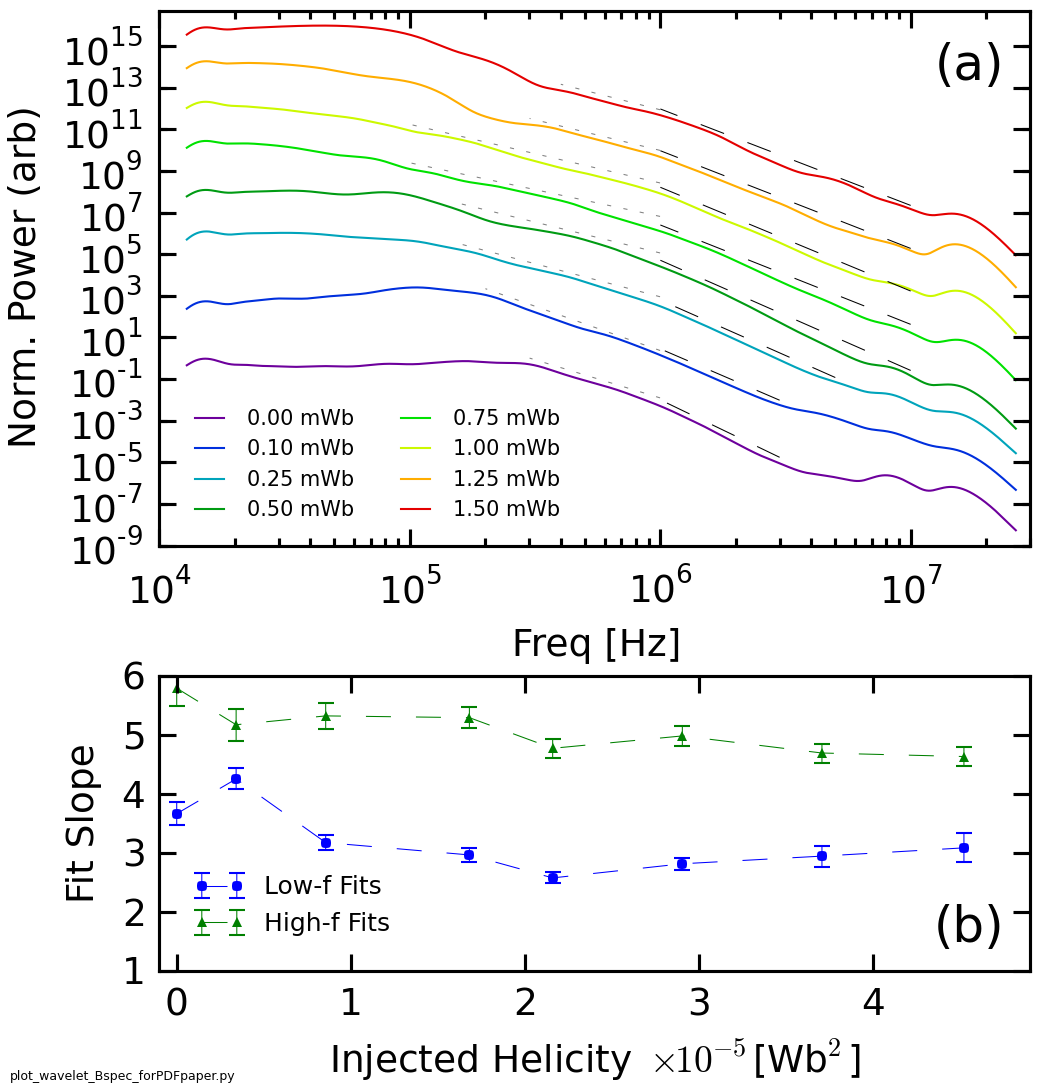
\includegraphics[width=8.5cm]{Br_spectra.png}}
\caption{\label{fig:Br_spectra} (a) Wavelet generated magnetic field fluctuation spectra for the radial direction ($B_{r}$), for each of the eight helicity states. The spectra are staggered in order to highlight the shape of each spectrum. (b) Fits for each spectra for either low or high frequencies. The width in frequency of each fit is indicated by the dashed lines in (a).}
\end{figure}

The calculation of spectra can be viewed as a second-order moment; since the results of this scan show no change for spectra, it is natural to seek potential changes at higher order moments. The amount of intermittency in the $\dot{B}(t)$ fluctuations for each helicity state does, however, appear to change. Figure~\ref{fig:Br_flatness} demonstrates how intermittency is determined through the measure of flatness. The PDF of increments is constructed by taking differences of values in a time signal---in this case, $\dot{B}_{r}$---separated by a time scale. Fig.~\ref{fig:Br_flatness}(a) shows the PDF of increments of a timeseries at 2$\times 10^{-5}$ Wb$^{2}$ of injected helicity for two different timescales: $0.15\mu s$ and $15\mu s$.  The PDF with small time scale shows a highly pointed PDF with broad, fat tails indicating large excursions from the mean value---or intermittency. This non-Gaussian behavior is highlighted when the PDFs are compared to a Gaussian curve. Dashed lines in Figure~\ref{fig:Br_flatness}(a) indicate the best-fit Gaussian to each distribution. The PDF with a large time scale increment clearly show a much more Gaussian distribution compared to its best fit. The level of intermittency for each scale can be quantified by taking the normalized fourth-order moment of the PDF---also called flatness or kurtosis. The flatness for each PDF at each time scale, as well as for each helicity state, is shown in Fig.~\ref{fig:Br_flatness}(b). Clearly, each state shows increasing flatness, and thus intermittency, with decreasing time scale. The flatness of a purely Gaussian distribution is indicated at F=3. Moreover, it is observed that the overall flatness of each curve increases as a function of helicity. In other words, the intermittency of the plasma increases with injected helicity---this is the main result of this paper.

\begin{figure}[!htbp]
\centerline{
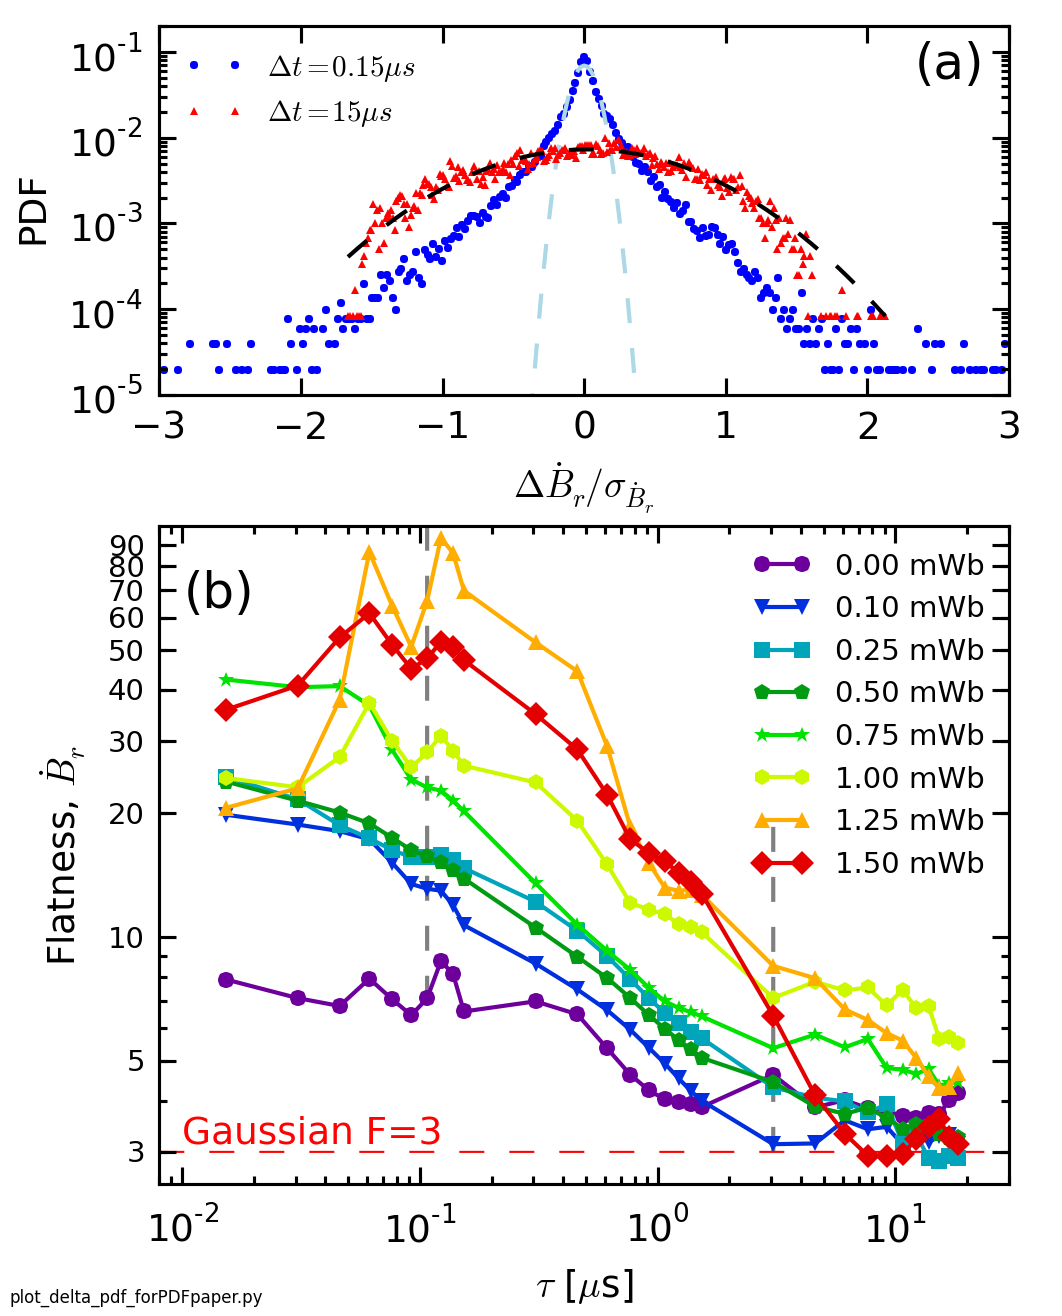
\includegraphics[width=8.5cm]{Br_flatness.png}}
\caption{\label{fig:Br_flatness} (a) PDFs for a long and short $\tau$ from data for $K_{B} = 2\times 10^{-5} Wb^{2}$ indicating the changing in intermittency with timescale. Dashed lines indicate the best-fit Gaussian curves for each PDF. (b) Flatness values for each timescale and each helicity state for the radial $\dot{B}$ component.}
\end{figure}

This change with helicity is summarized in Figure~\ref{fig:flatness_scaling}(a) where the calculated flatness of each curve in Fig.~\ref{fig:Br_flatness}(b) as well as those for $\dot{B}_{\theta}$ and $\dot{B}_{z}$ has been averaged between the scales indicated by the dashed gray lines: between $0.1\mu s$ and $3.0\mu s$, which approximately corresponds to a frequency range of 333kHz to 10MHz. The average flatness generally increases with helicity, although there is a brief reversal of trend at about 1$\times 10^{-5}$ Wb$^{2}$ before the curve begins to increase again.

\begin{figure}[!htbp]
\centerline{
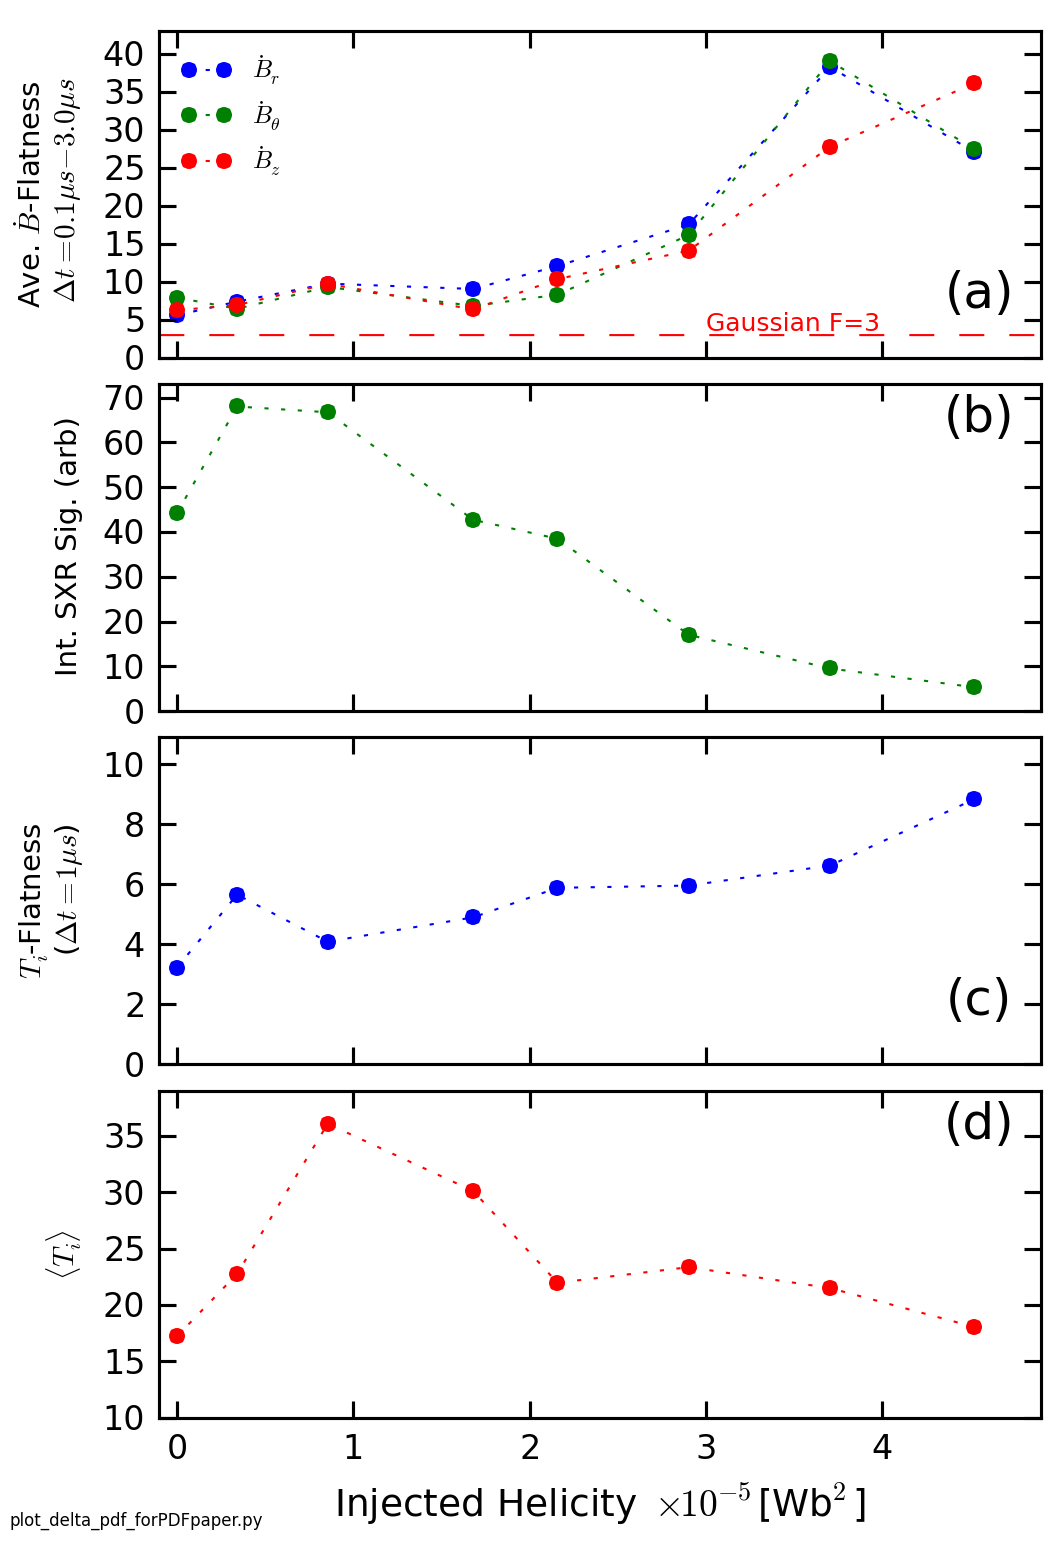
\includegraphics[width=8.5cm]{flatness_scaling.png}}
\caption{\label{fig:flatness_scaling} (a) Average flatness versus helicity. (b) Integrated soft X-ray signal versus helicity. (c) Flatness of $T_{i}$ time series versus helicity. (d) Average $T_{i}$ versus helicity.}
\end{figure}

While the physical origin of this observed intermittency and its trend with helicity is not completely understood in the context of this experiment, investigation of intermittency in space plasma yields some possible explanations. Simulations of MHD plasmas modeled after solar wind plasma with time series extracted in ways to match that of \textit{in-situ} satellite observation~\cite{Greco08,Greco09}, have indicated a correlation between intermittency and the passing of current sheets or reconnection sites. Past experiments on SSX have focused on observation of reconnection layers~\cite{Gray10,brown12}; thus, the experiment has a number diagnostics designed to measure signatures of reconnection including a set soft X-ray photo-diodes~\cite{chaplin09} to measure X-rays generated by fast electrons and an Ion Doppler spectrometer (IDS) system that measures bursts of ion temperature and flow~\cite{brown12}. Figure.~\ref{fig:flatness_scaling}(b-d) shows the output of these diagnostics for the same helicity scan and limited to the same time range as the turbulence data presented above. Soft X-ray measurement shows an initial increase in x-ray light going from zero to small amounts of helicity, but then a consistent decrease in radiation. Fig.~\ref{fig:flatness_scaling}(c) shows flatness of the ion temperature timeseries as a function of helicity constructed from PDF of increments with a timescale of $1\mu s$, the minimum time step available for the IDS system. Like, the flatness curve of $\dot{B}$, the ion temperature intermittency also increases with helicity. Meanwhile, the average, or background, ion temperature does not vary much, peaking slightly between 1 and 2$\times 10^{-5}$ Wb$^{2}$, but generally maintaining a value of between 20-25eV. 

Taken together, these trends can be viewed as evidence for a connection between intermittency and reconnection. The hypothesis is that increasing the injected helicity increases the number of reconnection sites during Taylor relaxation (more $T_{i}$) bursts but decreases their size (less X-ray light from electron acceleration). Unfortunately, this hypothesis cannot be fully tested without higher spatial resolution (current spectroscopy diagnostics are line-integrated) and better temporal resolution in the ion measurements. In addition to improving diagnostics, comparisons to simulation may help as is done in solar wind research.

This paper presents the observation of a clear change in the intermittent character of $\dot{B}$ fluctuations as a function of injected helicity while simultaneously showing little to no change in the energy transfer rate between scales as indicated by the turbulent power spectra. This discrepancy is perhaps an indication of the need to study higher order moments in turbulence analysis (i.e. 4th order Flatness vs 2nd order spectra) in order to fully flesh out modifications in turbulence~\cite{matthaeusVelli11}. The experiment also demonstrates a straightforward method for modifying the intermittency in a plasma for detailed study and highlights an advantage of turbulence research in an experimental setting as a complement to {\it in-situ} measurements and simulation. A possible connection to a physical mechanism was established through soft X-ray and IDS measurements, which suggested the intermittency is related to the spatial size of reconnection sites in the plasma. However, given the limitations of the current diagnostics, definitive conclusions cannot be made, but do provide impetus for further comparison to simulation.

Finally, since helicity observations have been made in many of the same turbulent plasmas that exhibit intermittency~\cite{goldstein94, ji95, telloni12}, a link between helicity and turbulent intermittency may be a useful metric for understanding turbulence in both space and experiment, including possible comparisons to the variation of intermittency as a function of solar distance~\cite{greco12} as well as differences between confinement regimes in fusion devices.

\providecommand{\noopsort}[1]{}\providecommand{\singleletter}[1]{#1}%
\begin{thebibliography}{99}

\bibitem{frisch95}Frisch, U. 1995, {\it Turbulence} (Cambridge: Cambridge Univ. Press)

\bibitem{sorrisovalvo99}Sorriso-Valvo, L. {\it et al.} Geophys. Res. Lett. {\bf 26}, 1801–1804 (1999).

\bibitem{wan12}Wan, M. {\it et al.} ApJ. {\bf 744} 177 (2012).

\bibitem{sorrisovalvo01}Sorriso-Valvo, L. {\it et al.} Planet. Space Sci. {\bf 49}, 1193–1200 (2001).

\bibitem{marrelli05}Marrelli, L. {\it et al.} Phys. Plasmas. {\bf 12}, 030701 (2005).

\bibitem{Greco08}Greco, A. {\it et al.} Geophys. Res. Lett. {\bf 35}, L19111 (2008).

\bibitem{Greco09}Greco, A. {\it et al.}, ApJ {\bf 691}, L111 (2009).

\bibitem{Wan09}Wan, M. {\it et al.} Phys. Plasmas {\bf 16}, 080703 (2009).

\bibitem{Servidio11b}Servidio, S. {\it et al}, J. Geophys. Res. {\bf 116}, A09102 (2011).

\bibitem{Gray13}T. Gray, M. R. Brown, and D. Dandurand. Phys. Rev. Lett. {\bf 110}, 085002 (2013). 

\bibitem{schaffner14}D.A. Schaffner {\it et al.} Turbulence analysis of an experimental flux rope plasma. Submitted to Plas. Phys. Cont. Fusion. (2014).

\bibitem{Taylor86}Taylor, J.B. Rev. Mod. Phys. {\bf 58}, 741 (1986).

\bibitem{Matthaeus80}Matthaeus,W.H. and Montgomery,D. Ann. N.Y. Acad. Sci. {\bf 357}, 203 (1980).

\bibitem{torrence98}Torrence, C. and Compo, G.P. Bull. Am. Meteorol. Soc. {\bf 79}, 6178 (1998).

\bibitem{clauset09}Clauset, A., Rohilla Shalizi, C. and Newman, M.E.J. SIAM Rev. {\bf 51}, 661703 (2009).

\bibitem{Gray10}Gray,T. {\it et al.} Phys. Plasmas {\bf 17}, 102106 (2010).

\bibitem{chaplin09}Chaplin, V.H., {\it et al.} Phys. Plasmas {\bf 16} 042505 (2009).

\bibitem{brown12}Brown, M.R. {\it et al.} Phys. Plasmas {\bf 19} 080704 (2012).

\bibitem{goldstein94}Goldstein, M.L., Roberts, D.A. and Fitch, C.A. Jour. Geo. Res. {\bf 99} 11519-11538 (1994).

\bibitem{ji95}Ji, H., Prager, S.C. and Sarff, J.S. Phys. Rev. Lett. {\bf 74} 2945 (1995).

\bibitem{telloni12}Telloini, D. {\it et al.}. ApJ. {\bf 751} 19 (2012).

\bibitem{matthaeusVelli11}Matthaeus, W.H. and Velli, M. Space Sci. Rev. {\bf 160} 145-168 (2011).

\bibitem{greco12}A. Greco {\it et al.} ApJ. {\bf 749} 105 (2012).

\end{thebibliography}

\end{document}

